\documentclass{beamer}

%\usepackage{beamerthemesplit}
\usecolortheme{crane}
\usepackage{graphicx}
\usepackage{listings}
\usepackage{verbatim}
\usepackage{ctable}
\usepackage{siunitx}
\usepackage{fontspec}
\setmonofont{DejaVu Sans Mono}

\lstset{language=C++,basicstyle=\ttfamily}
\lstset{extendedchars=false,showstringspaces=false}

\title{ROI Model Draft Overview}
\author{Roger Leigh}
\date{6th November 2012\\University of Dundee}

\begin{document}

\frame{
  \titlepage
  \begin{center}
      
\includegraphics[width=0.35\textwidth]{../images/dundee}\hfill
      \parbox[b]{0.5\textwidth}{
        \hfill
\includegraphics[width=0.45\textwidth]{../images/scijava}\\
        \smallskip
        \hfill
\includegraphics[width=0.45\textwidth]{../images/ome}
      }
  \end{center}
}

\section*{Overview}
\frame{
\frametitle{Overview}
\tableofcontents
}

\frame{
  \frametitle{What is a ROI?}
  \LARGE
  \begin{description}
  \item[ROI] Region of interest.  A subset of samples within an image.
    This is specified by the boundary or surface of the object.
  \item[Shape] Geometric shape or mask.  A shape is a geometric
    primitive or bitmask.  A ROI is composed of one or more shapes.
  \end{description}
}

\section{Existing models}

\frame{
\frametitle{Existing models: ImageJ}
\begin{center}
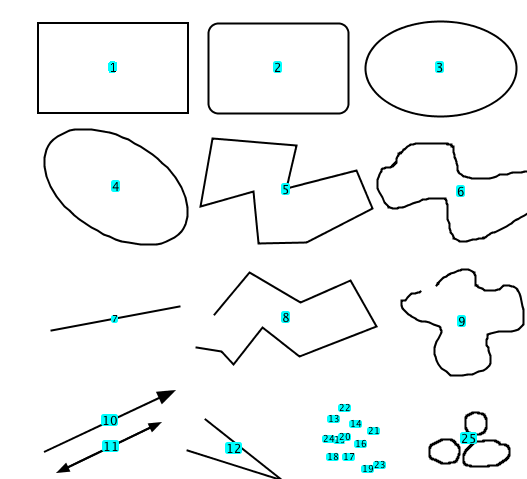
\includegraphics[width=0.75\textwidth]{../reference/imagej/rois}
\end{center}
}

\frame{
\frametitle{Existing models: Insight}
\begin{center}
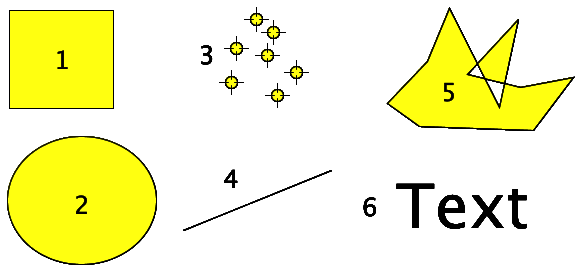
\includegraphics[width=\textwidth]{../reference/insight/rois}
\end{center}
}

\frame{
\frametitle{Existing models: Icy}
\begin{center}
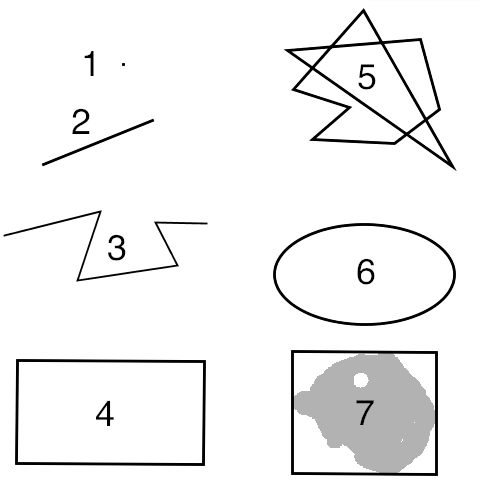
\includegraphics[width=0.7\textwidth]{../reference/icy/rois}
\end{center}
}

\frame{
\frametitle{Existing models: Volocity}
\begin{center}
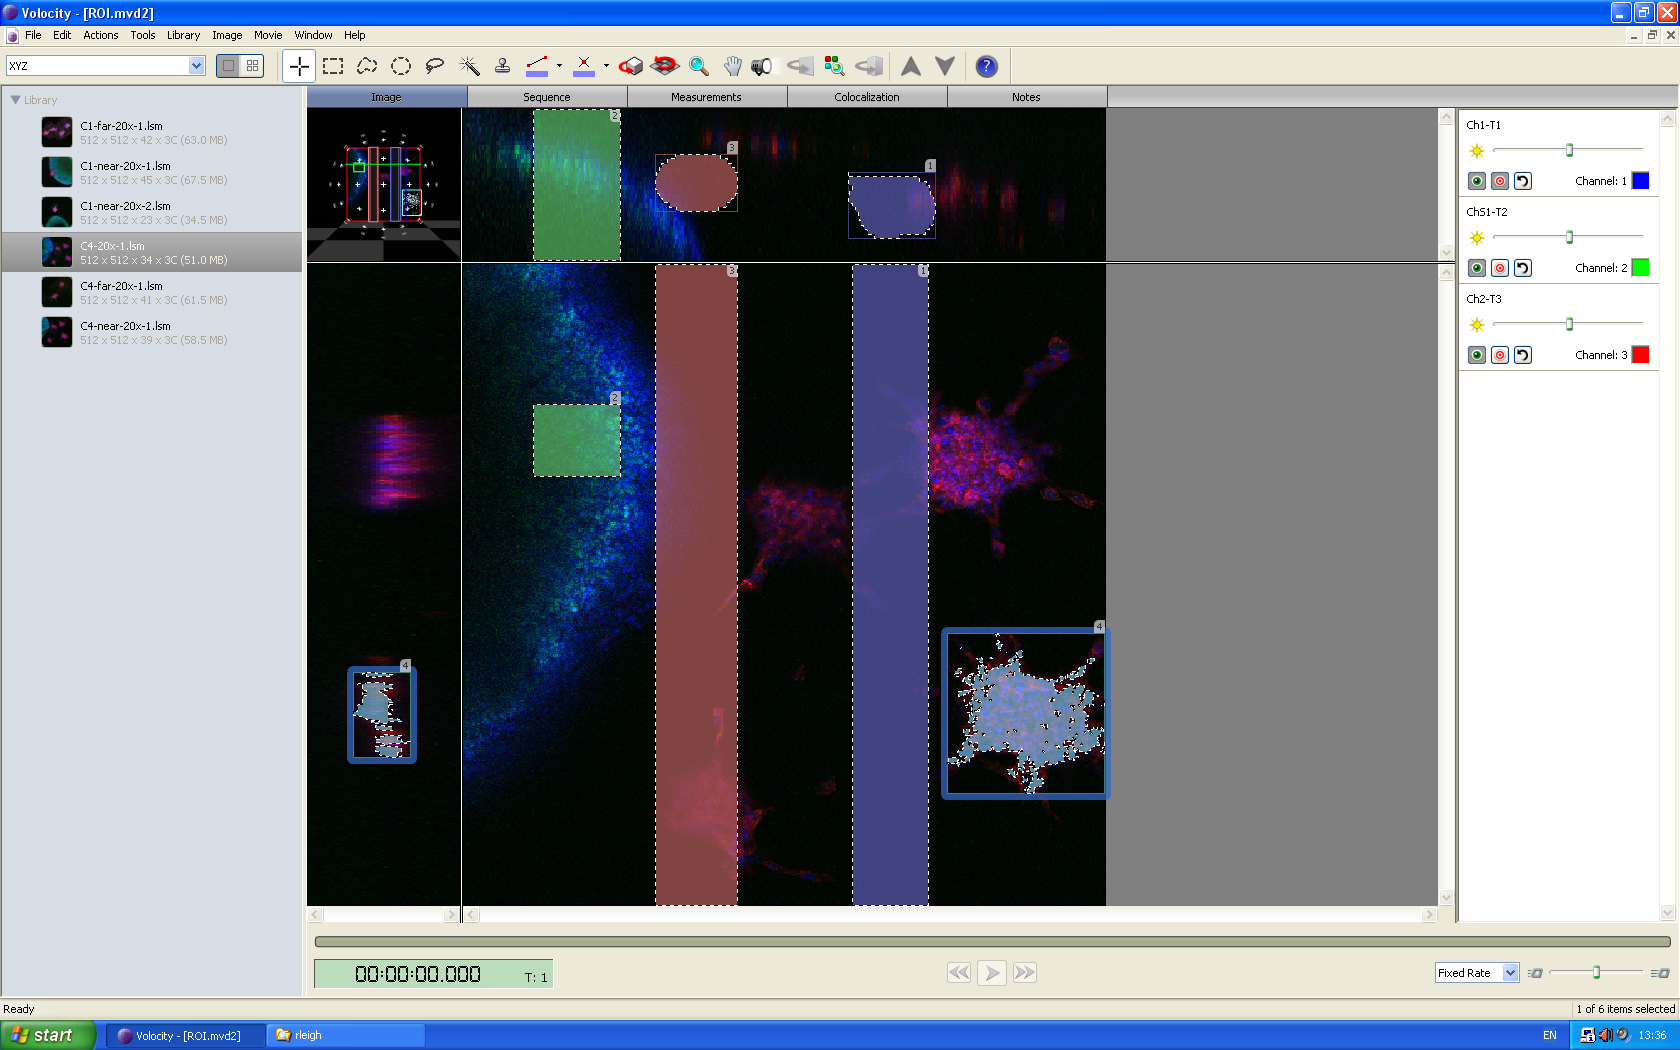
\includegraphics[width=\textwidth]{../reference/volocity/volocity1}
\end{center}
}

\frame{
\frametitle{Existing models: Volocity}
\begin{center}
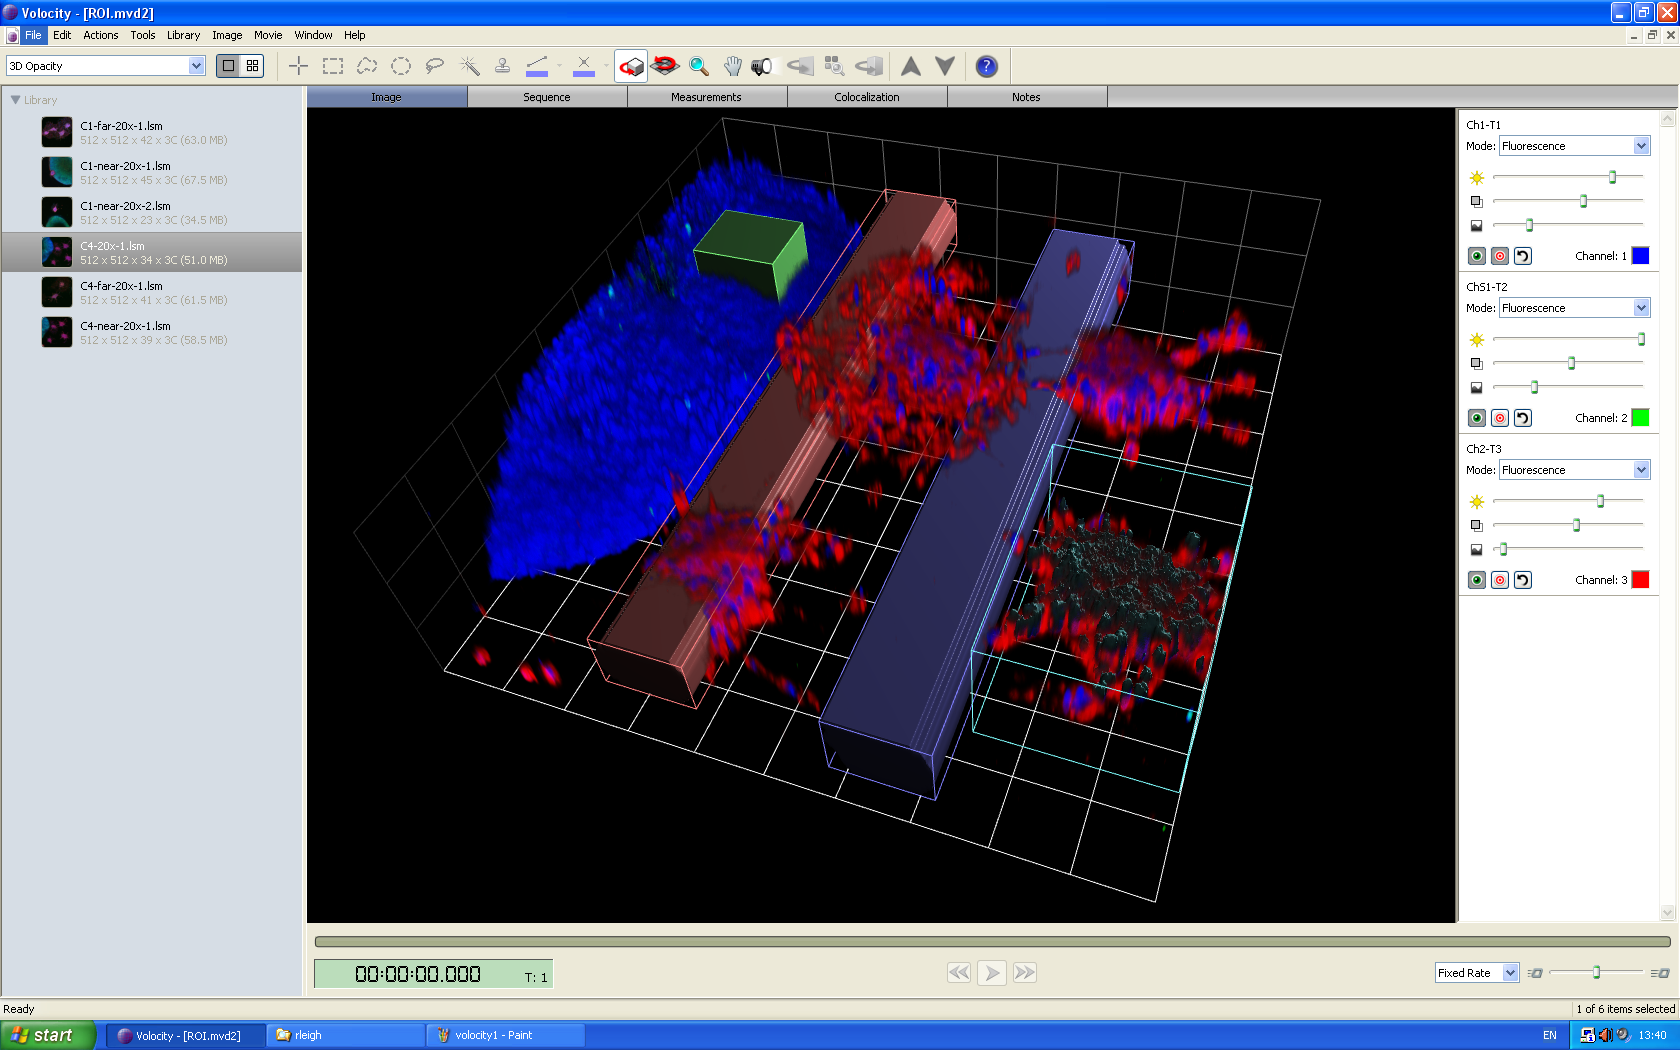
\includegraphics[width=\textwidth]{../reference/volocity/volocity2}
\end{center}
}

\frame{
\frametitle{Existing models: Volocity}
\begin{center}
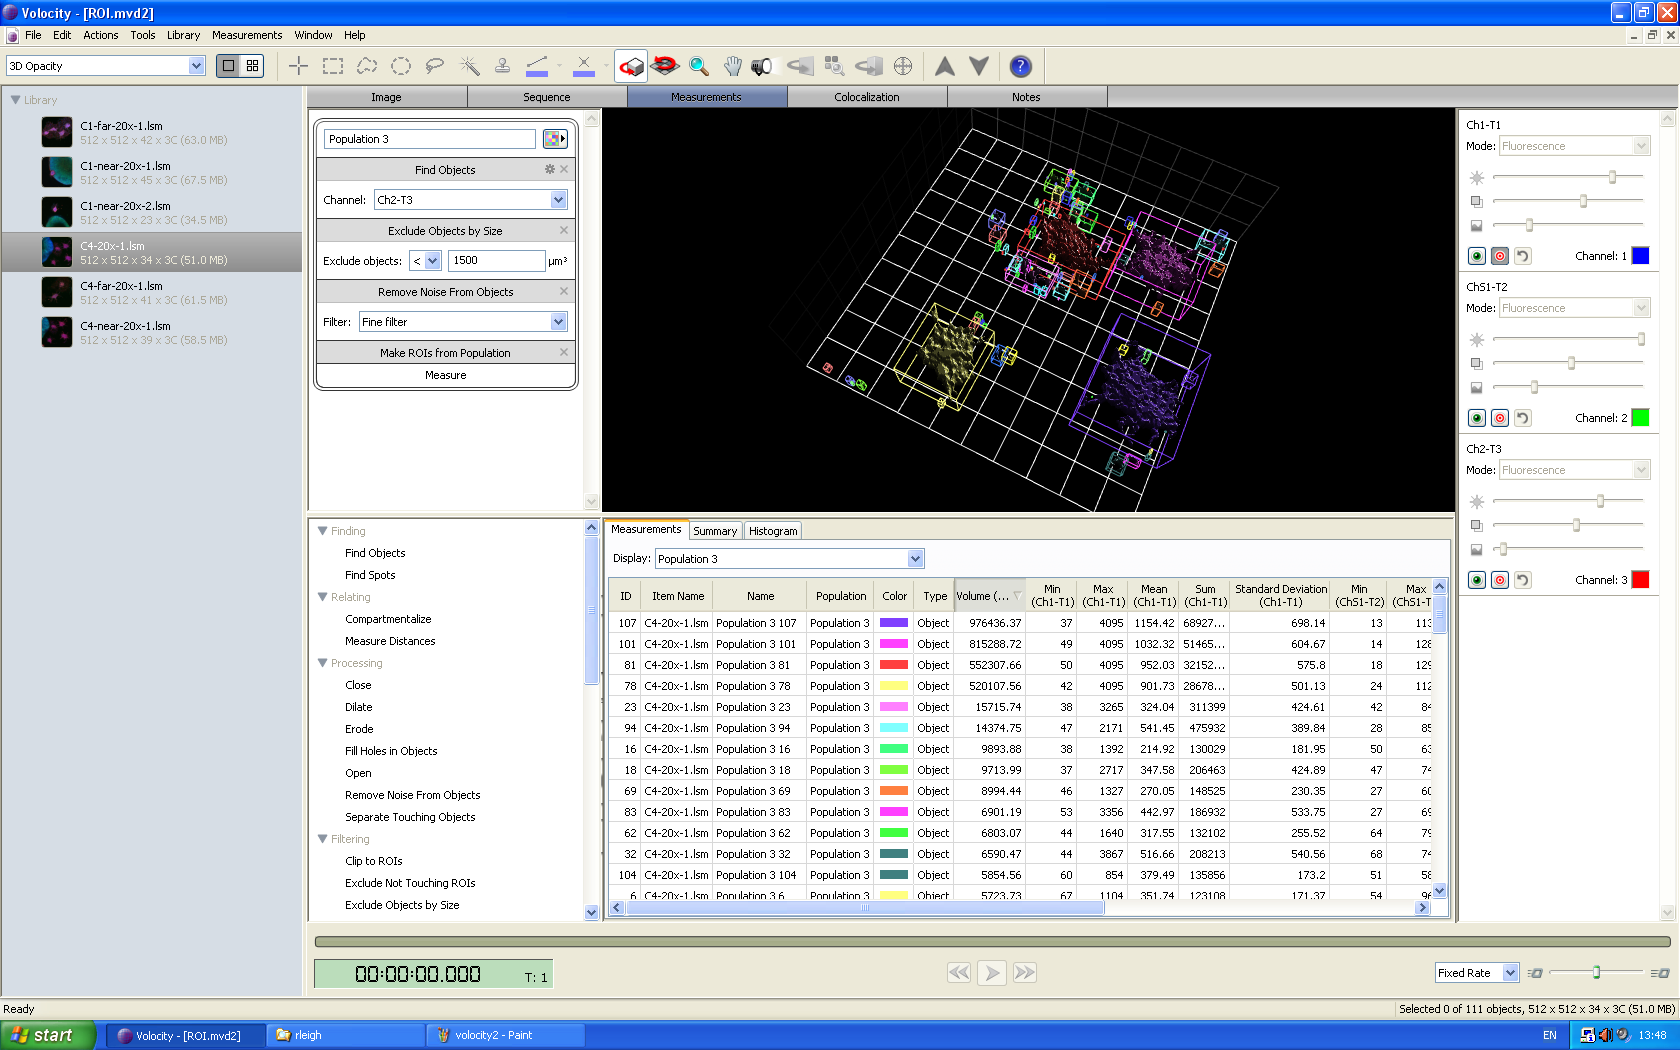
\includegraphics[width=\textwidth]{../reference/volocity/volocity3}
\end{center}
}

\frame{
\frametitle{Existing models: Volocity}
\begin{center}
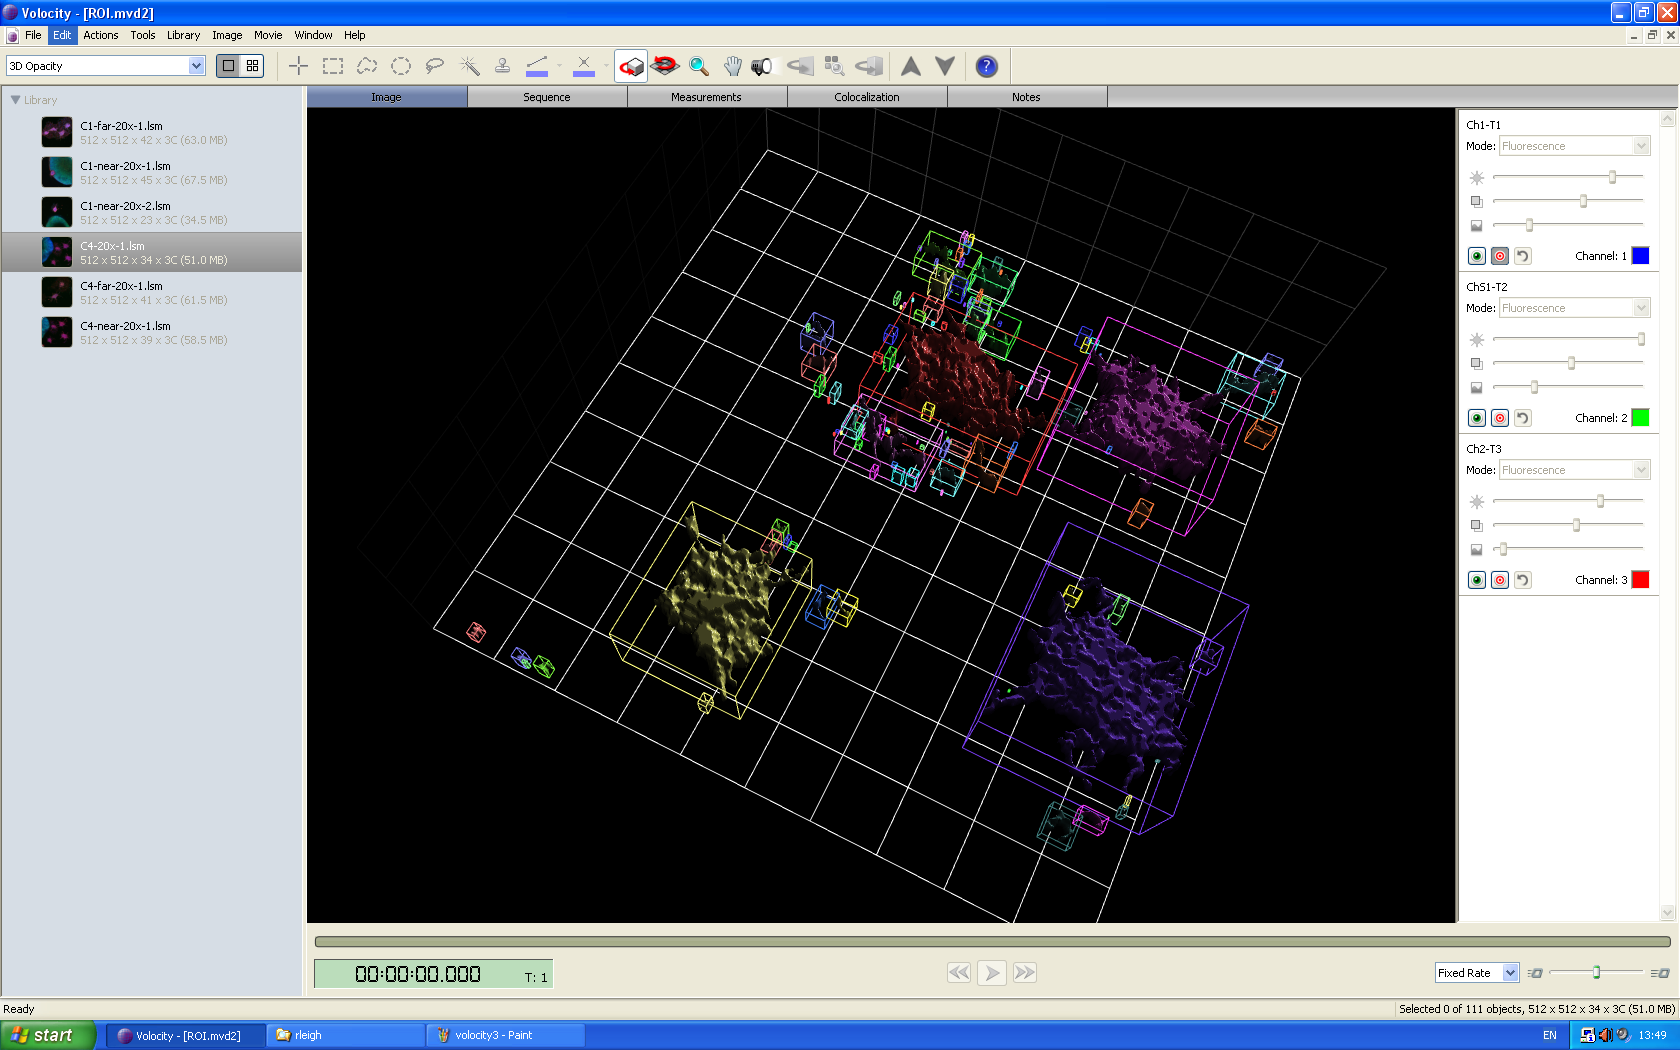
\includegraphics[width=\textwidth]{../reference/volocity/volocity4}
\end{center}
}

\section{Model draft}

\frame{
\frametitle{The draft specification}
\begin{itemize}
\item This is a work in progress
\item Everything is changeable, nothing is fixed
\item In git
  \begin{itemize}
  \item \url{git://github.com/scijava/roi-model.git}
  \end{itemize}
\item Specification text
  \begin{itemize}
  \item Sphinx markup
  \item \texttt{*.rst}
  \end{itemize}
\item Storage/interface definitions
  \begin{itemize}
  \item Tab-separated tabular data
  \item \texttt{spec/*.txt}
  \end{itemize}
\item Code/specification generator
  \begin{itemize}
  \item \texttt{genspec}, \texttt{python/*.py}
  \end{itemize}
\item Java/C++/other reference implementations (TBD)
\end{itemize}
}

\frame{
\frametitle{The draft specification}
\begin{itemize}
  \item This specification addresses:
    \begin{itemize}
      \item Describing ROIs
      \item Serialising ROIs for storage and exchange
      \item Converting ROIs to iterable entities
      \item Drawing ROIs
      \item Editing ROIs
    \end{itemize}
  \item This specification \emph{does not} address:
    \begin{itemize}
      \item ROI-ROI links for tracking, and other high-level ROI
        inter-relationships.
      \item A directed graph of ROI-ROI links would be a potential
        solution.
    \end{itemize}
\end{itemize}
}


\section{Shapes}

\subsection{Example: A sphere}

\frame{
\frametitle{Describing a sphere}
\begin{center}
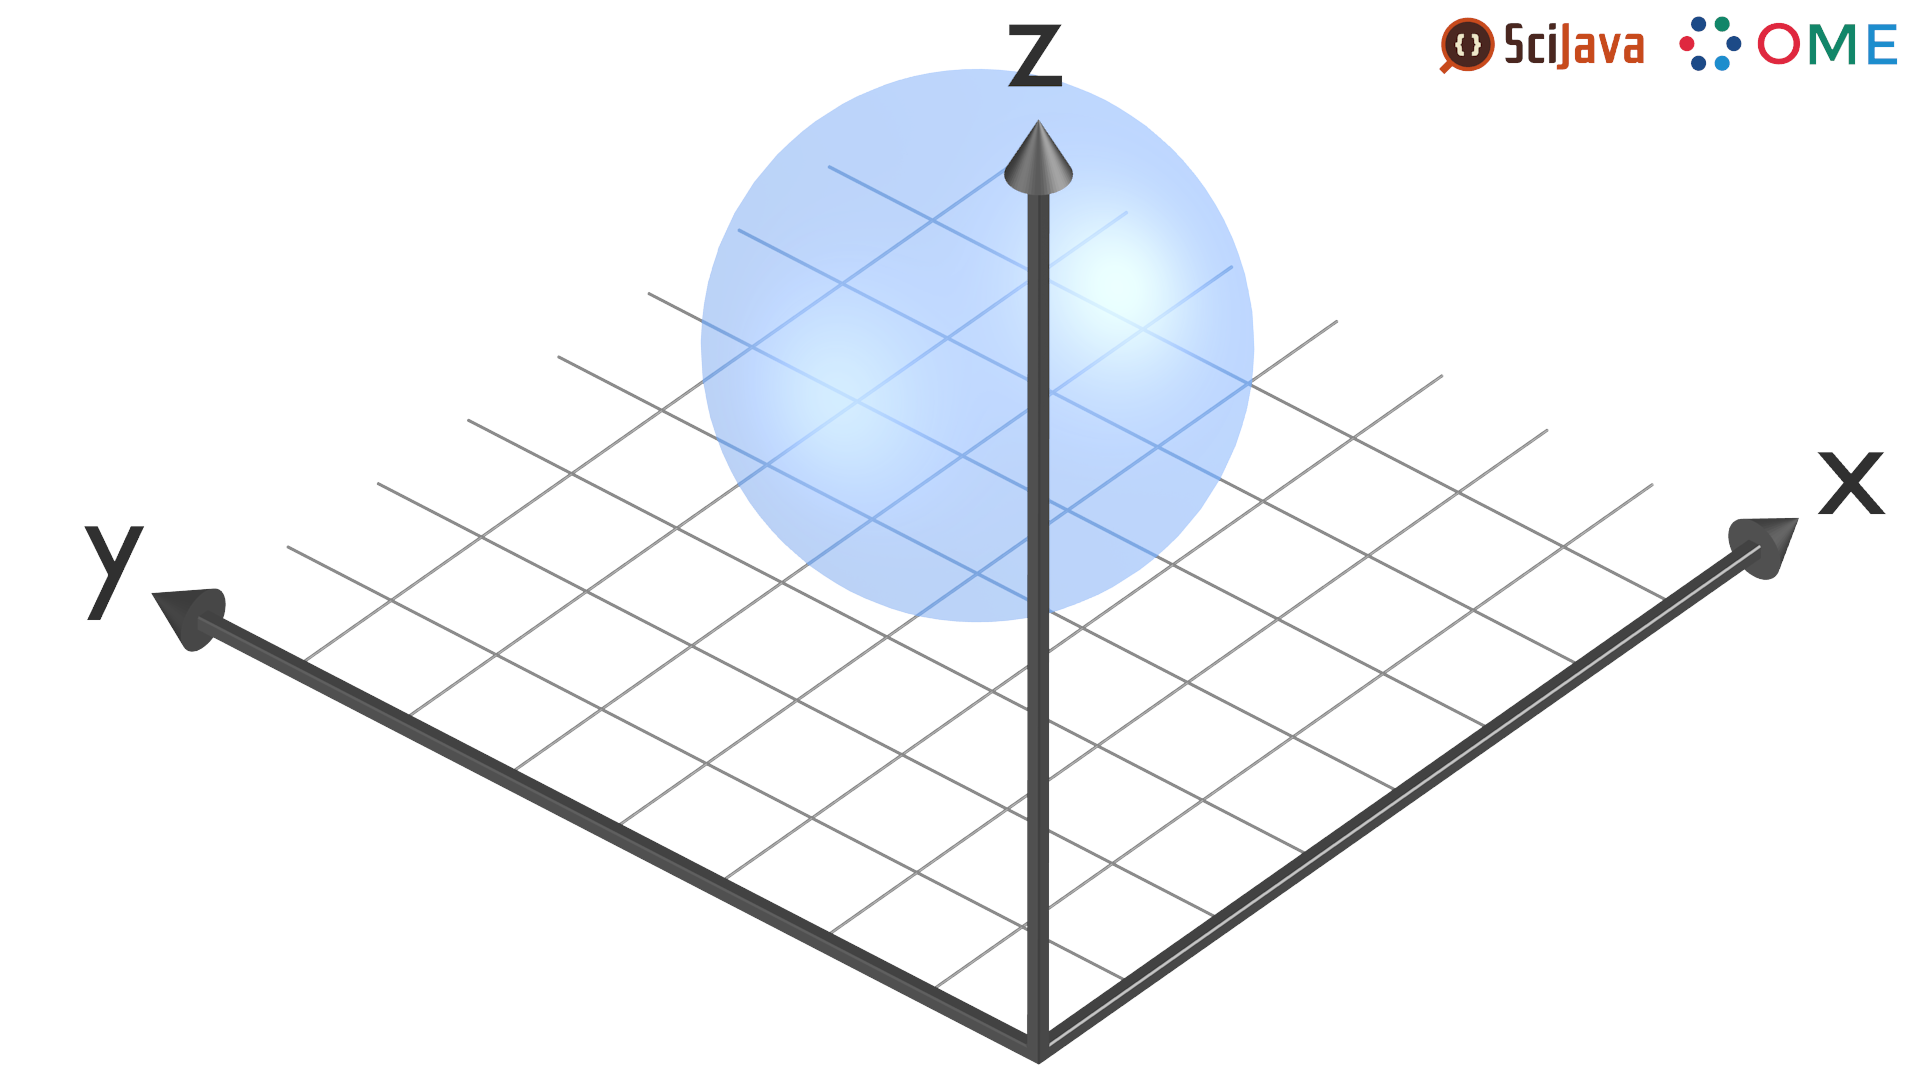
\includegraphics[width=\textwidth]{../images/3Dsphere}
\end{center}
}

\frame{
\frametitle{Describing a sphere: centre and radius}
\begin{center}
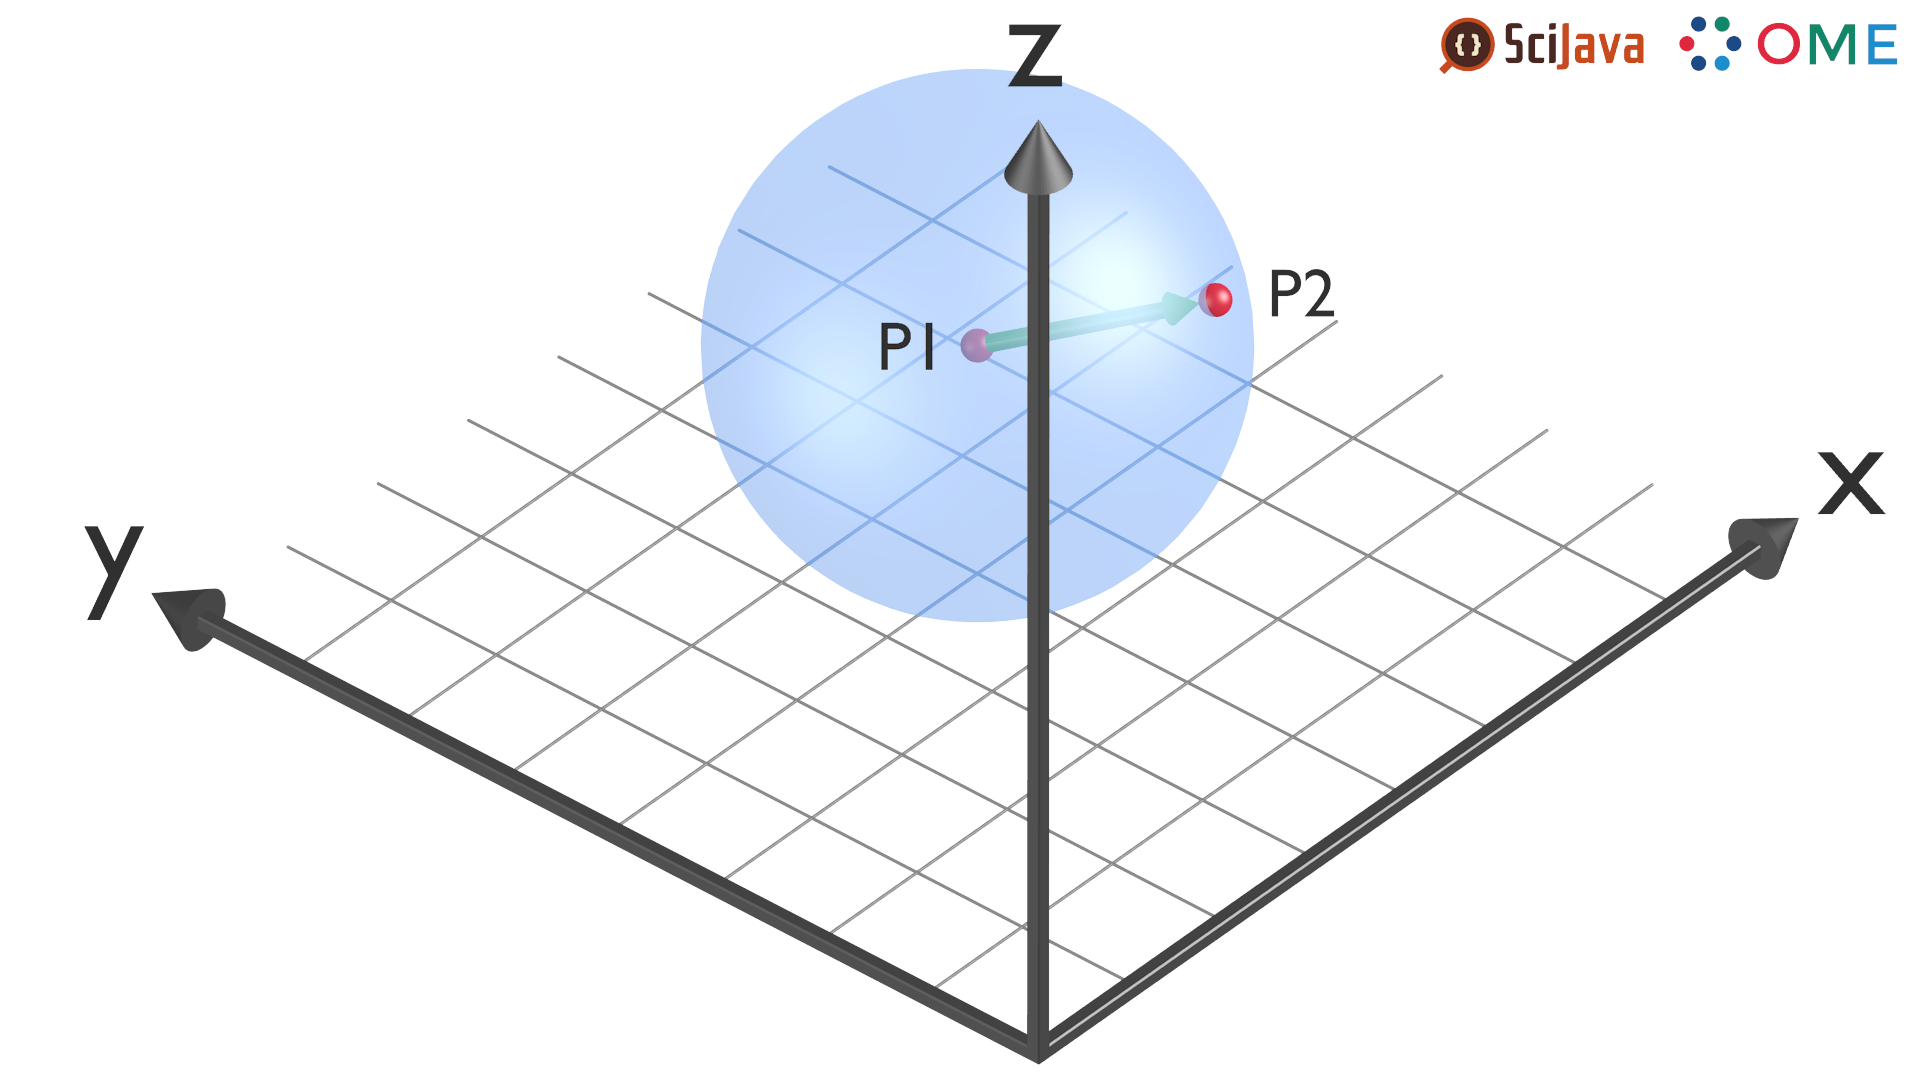
\includegraphics[width=\textwidth]{../images/3DspherePPR1.png}
\end{center}
}

\frame{
\frametitle{Describing a sphere: centre and radius}
\begin{center}
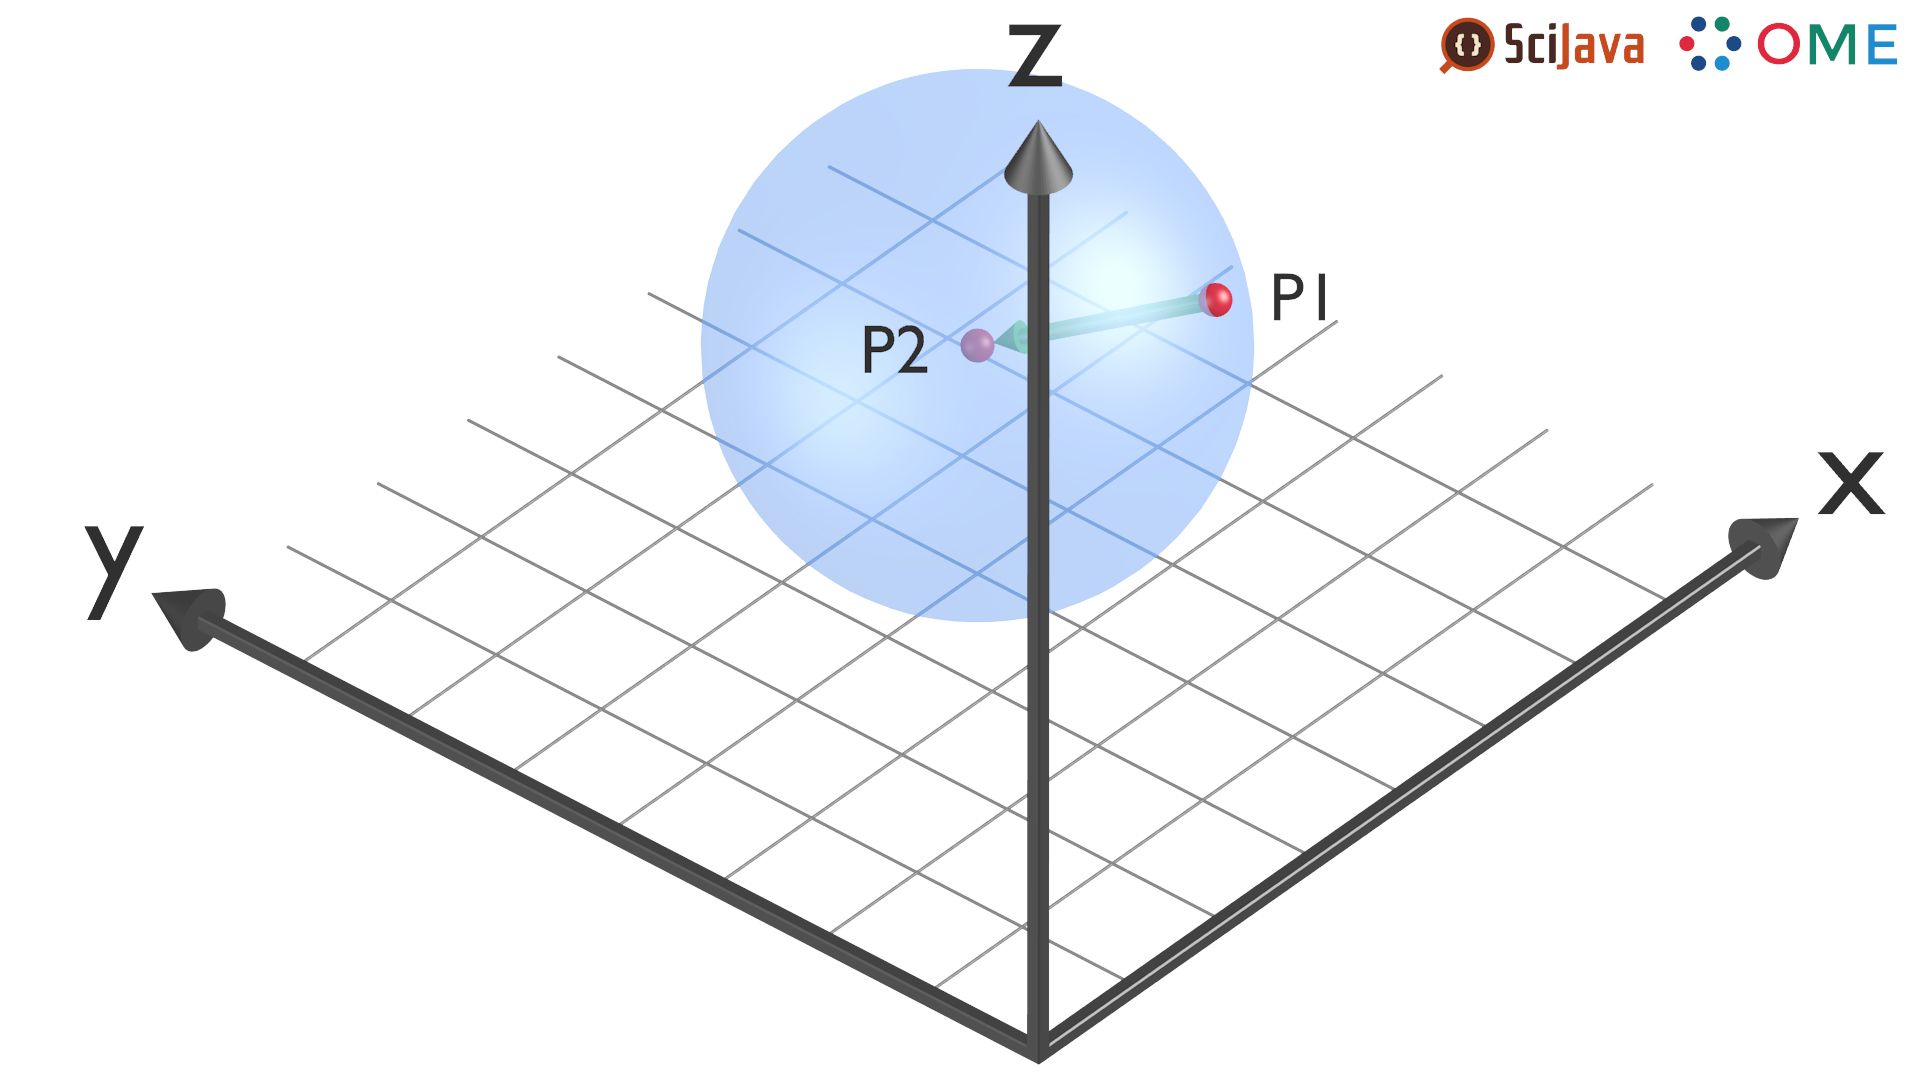
\includegraphics[width=\textwidth]{../images/3DspherePPR2.png}
\end{center}
}

\frame{
\frametitle{Describing a sphere: centre and radius}
\begin{center}
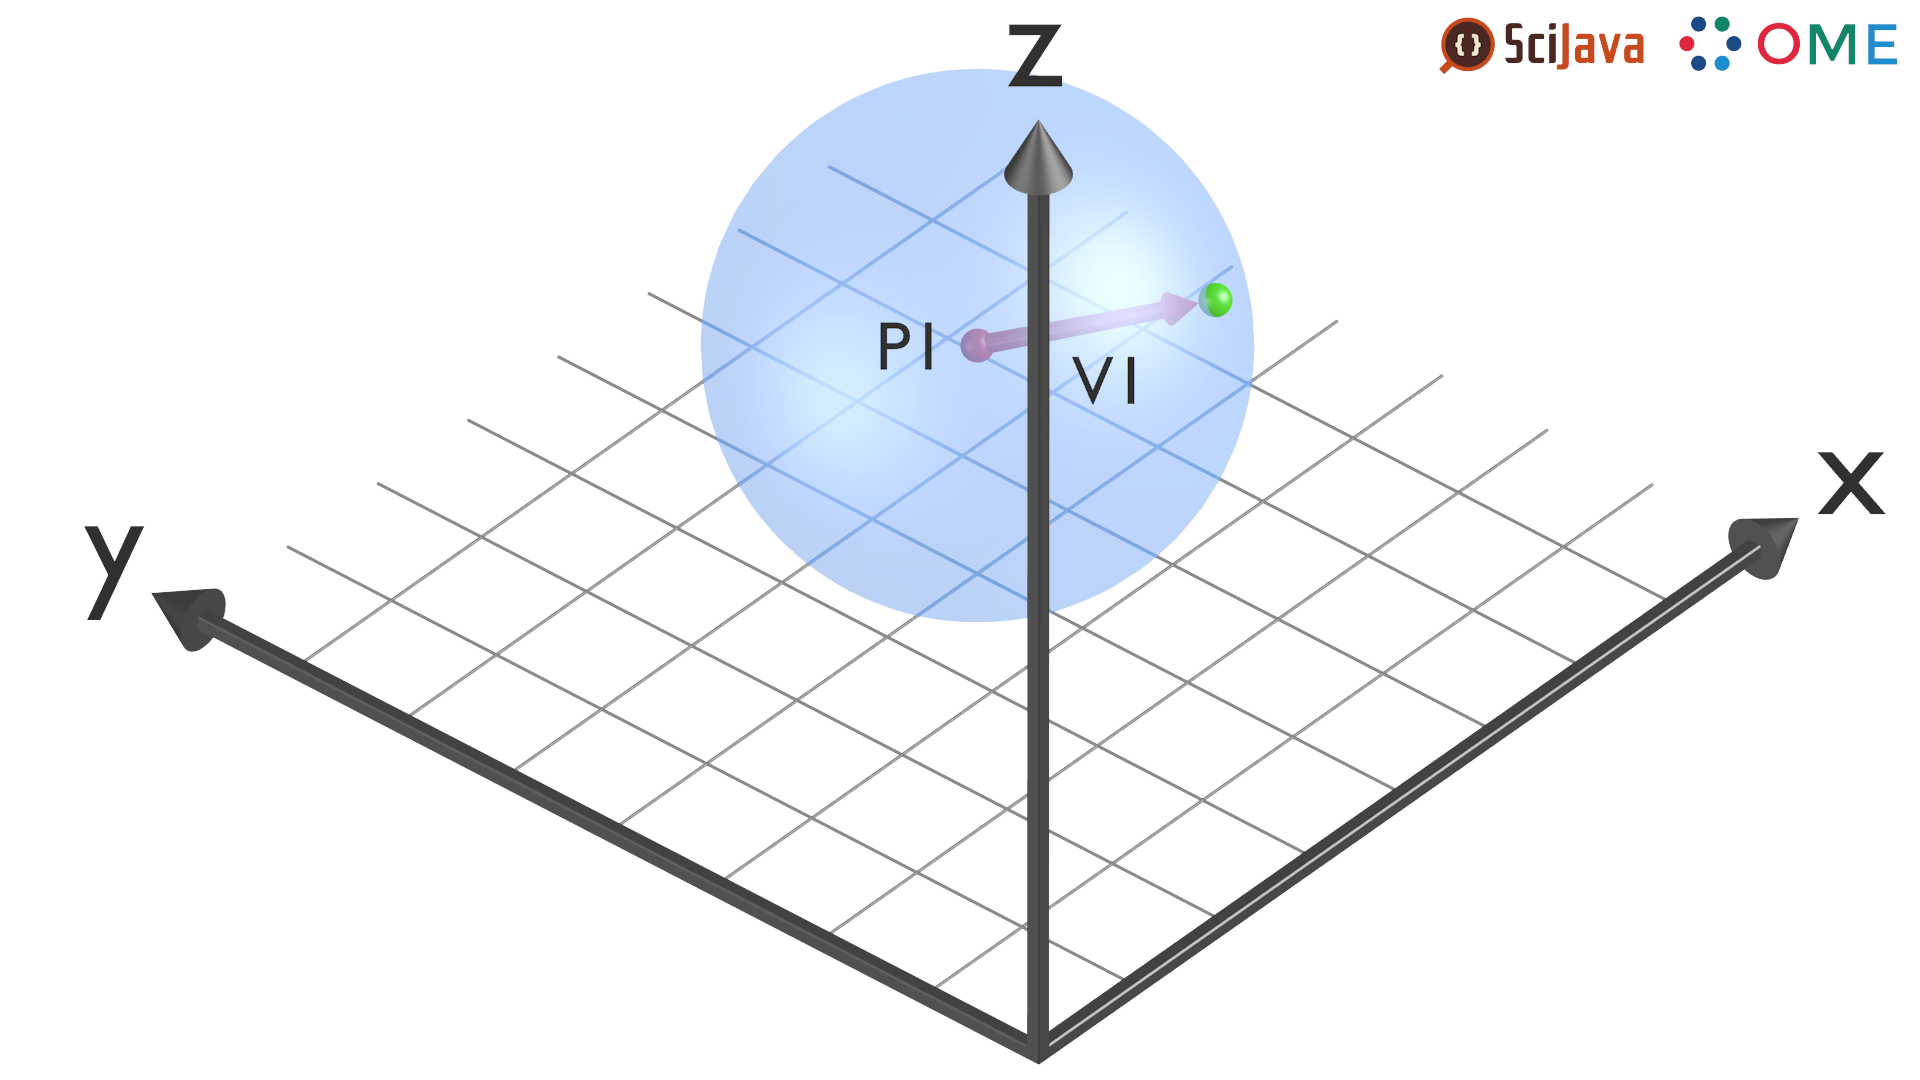
\includegraphics[width=\textwidth]{../images/3DspherePVR1.png}
\end{center}
}

\frame{
\frametitle{Describing a sphere: centre and radius}
\begin{center}
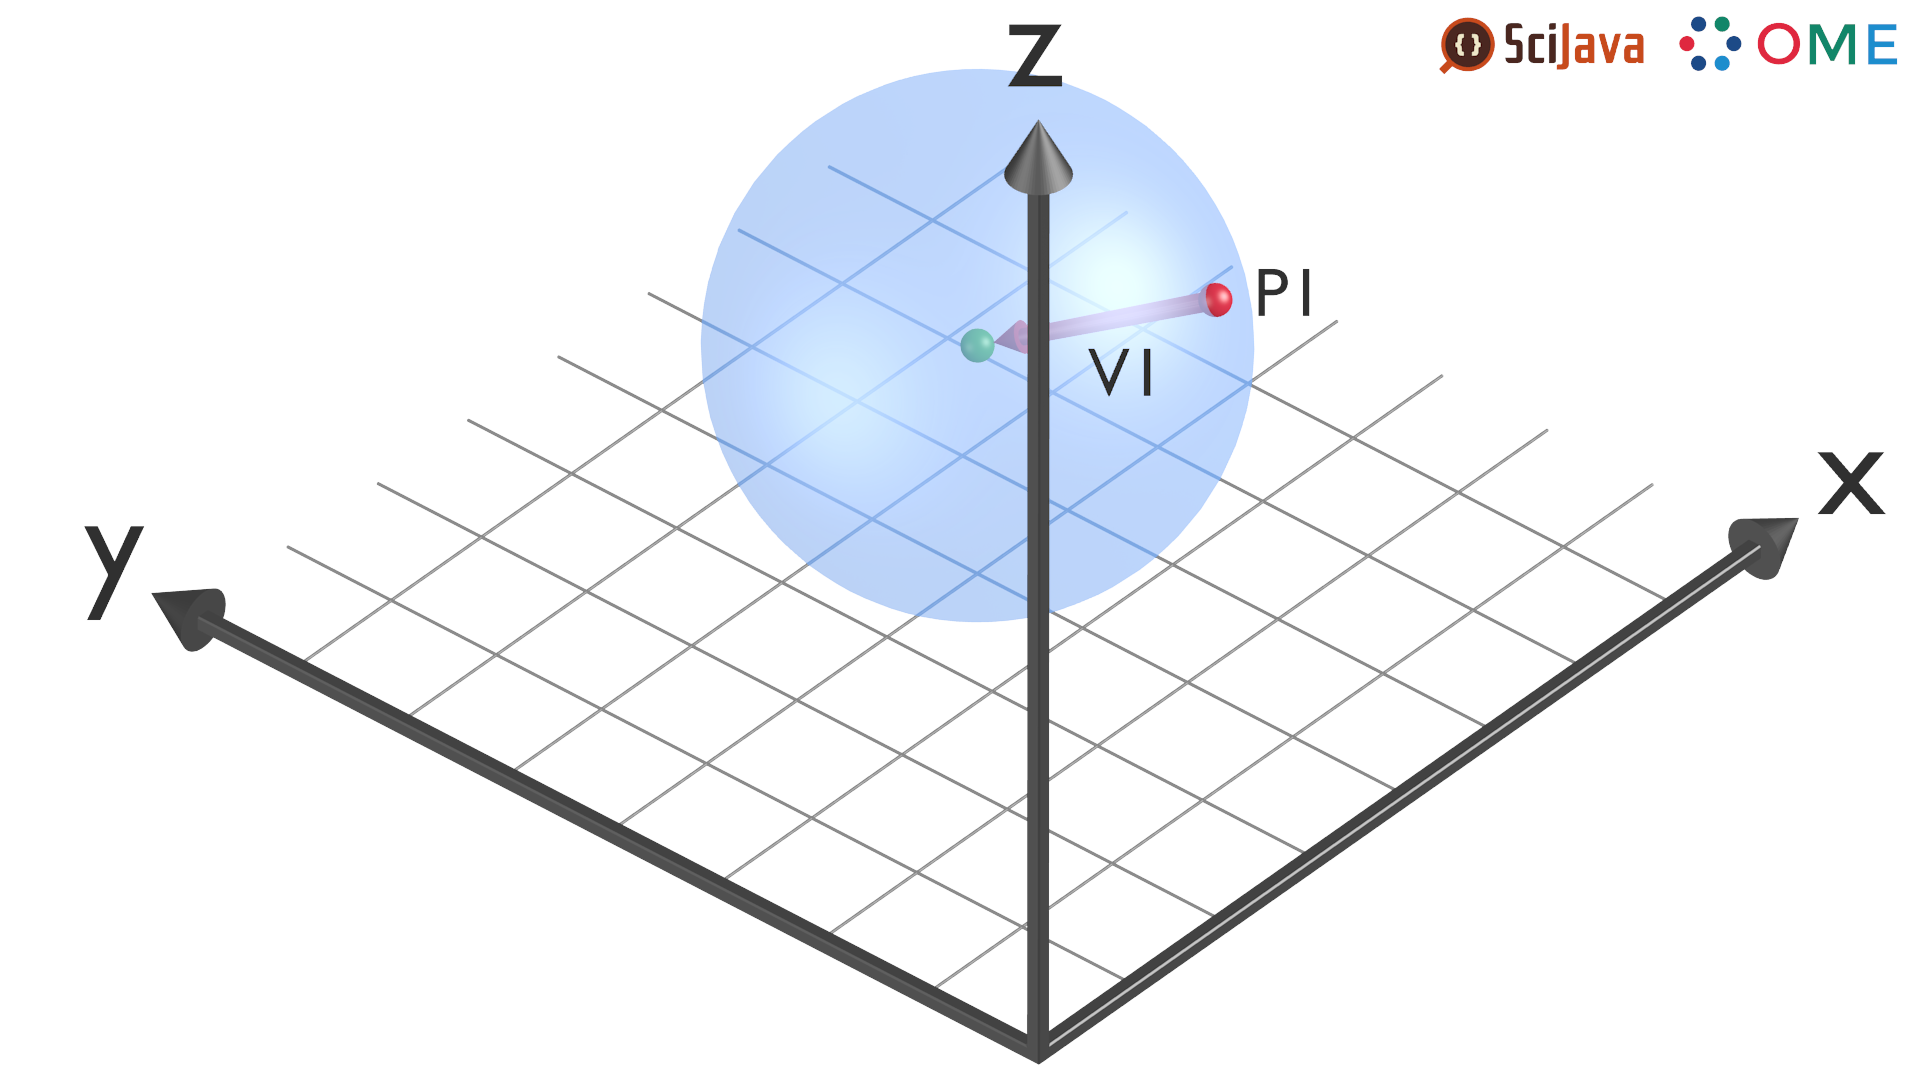
\includegraphics[width=\textwidth]{../images/3DspherePVR2.png}
\end{center}
}

\frame{
\frametitle{Describing a sphere: diameter}
\begin{center}
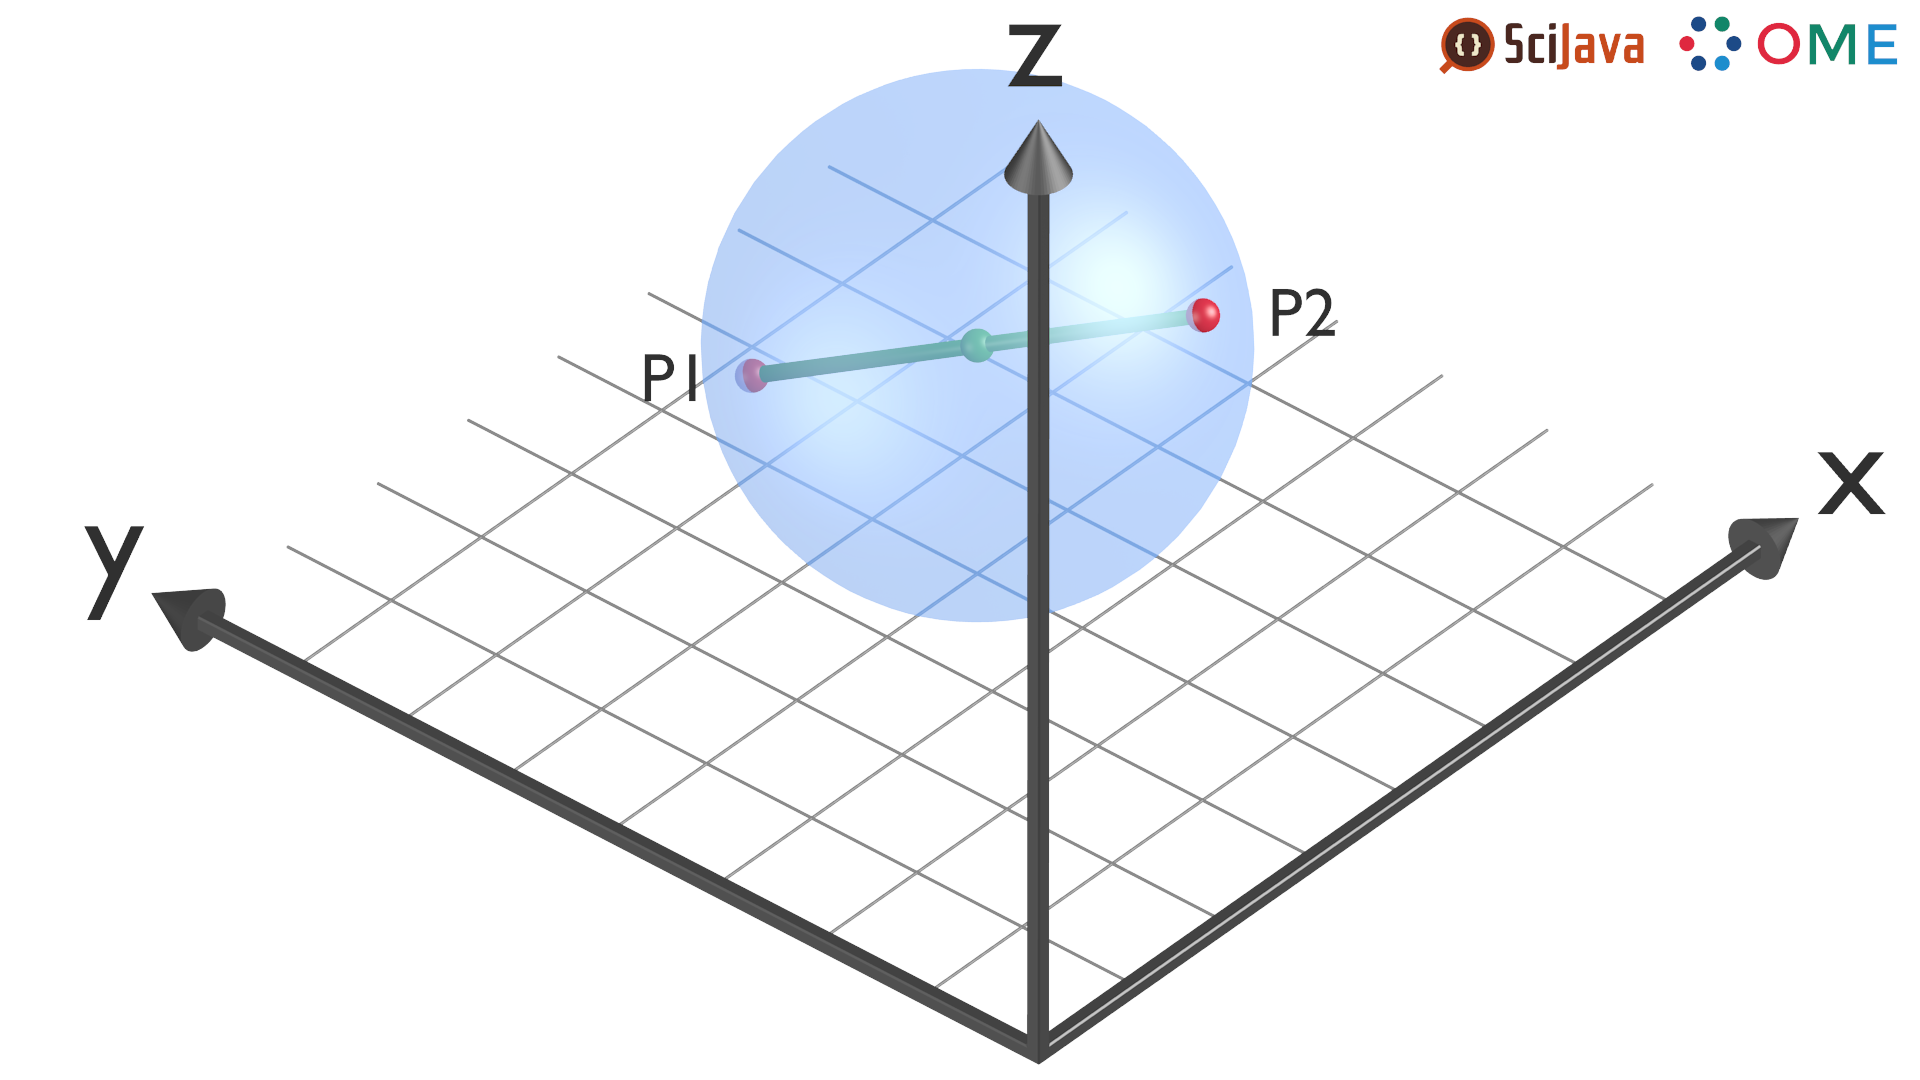
\includegraphics[width=\textwidth]{../images/3DspherePPD.png}
\end{center}
}

\frame{
\frametitle{Describing a sphere: surface}
\begin{center}
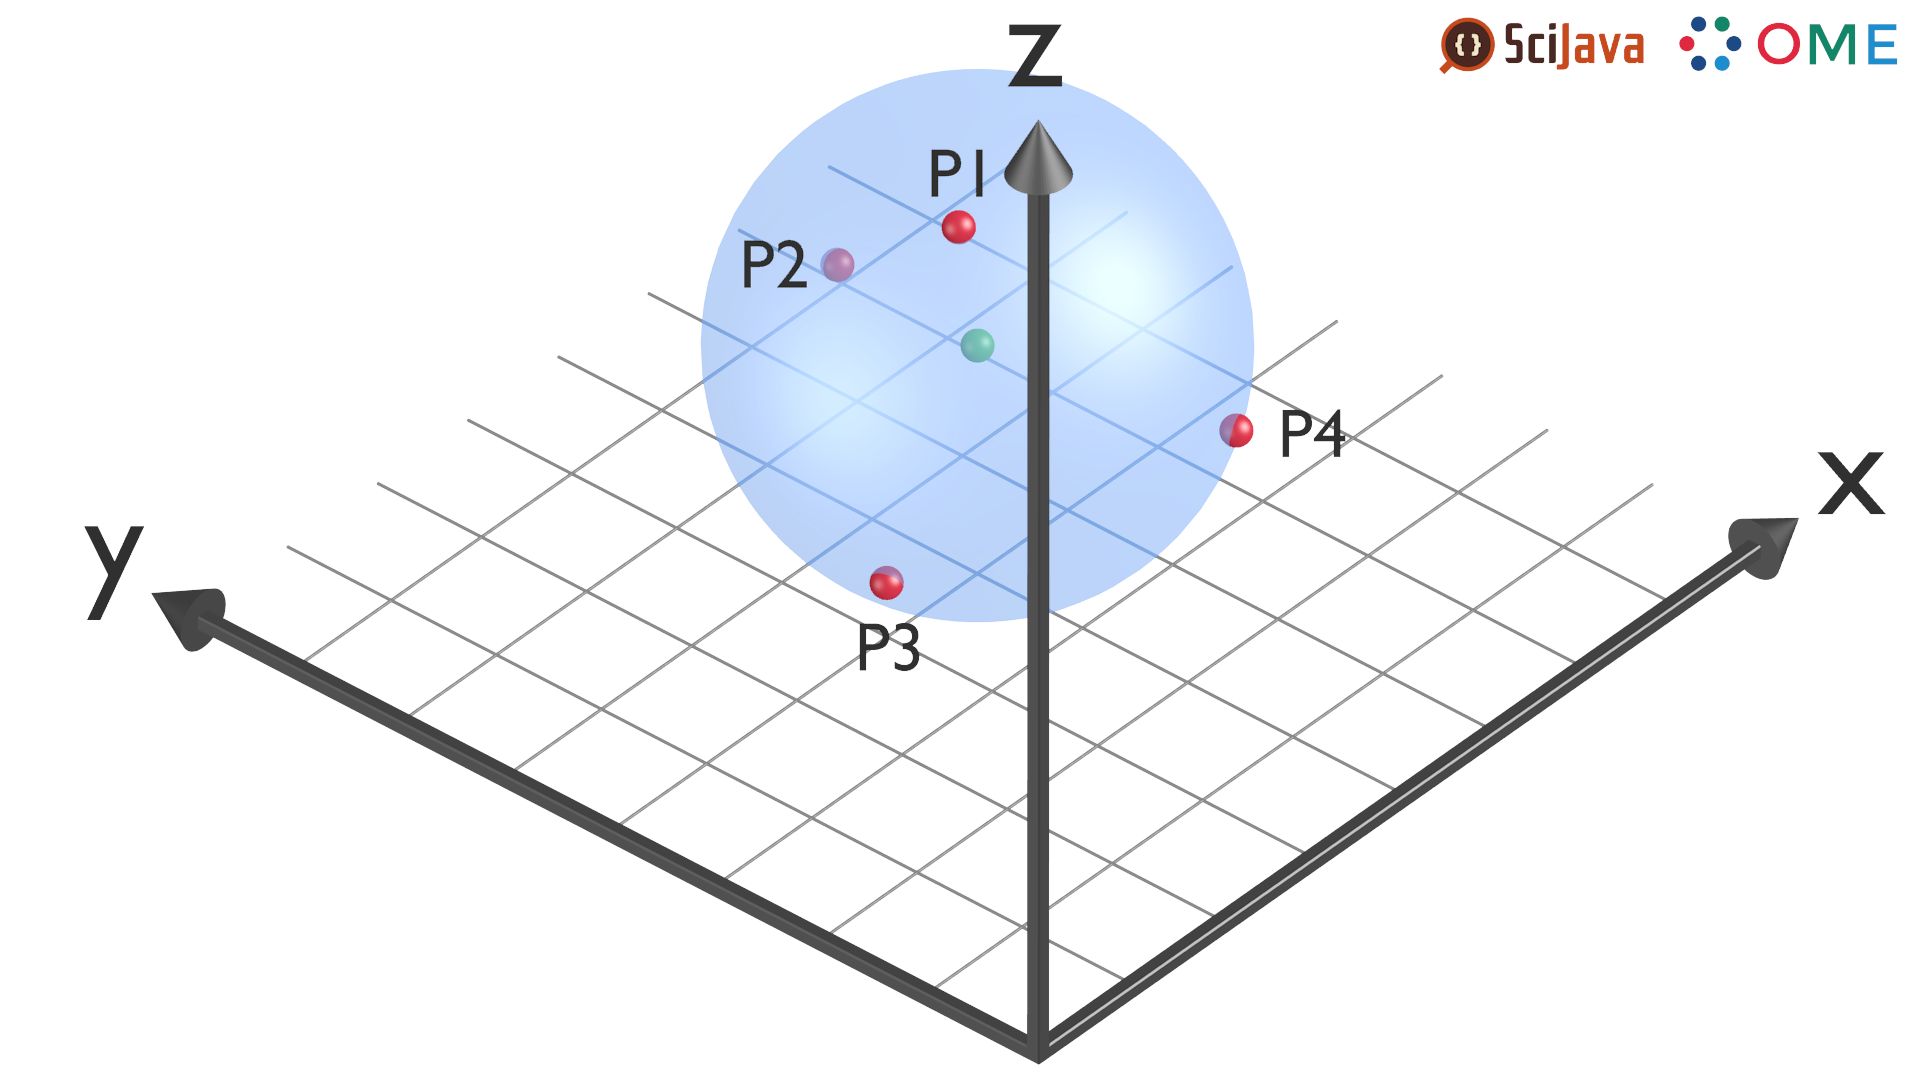
\includegraphics[width=\textwidth]{../images/3DspherePPPP.png}
\end{center}
}

\subsection{Shapes and representations}

\frame{
\frametitle{A region of interest}
\begin{center}
\begin{itemize}
\item Shape
  \begin{itemize}
    \item 3D geometric form
    \item 2D shapes are described by a 1 pixel thick 3D shape
    \item nD values or range
  \end{itemize}
\item Representation
  \begin{itemize}
  \item How the shape is described
  \item A shape may have one or more representations
  \item One representation is the default or canonical representation for each shape
  \end{itemize}
\item Serialisation
  \begin{itemize}
  \item A ROI is fully described by a shape ID, representation ID and
    the representation data (points, vectors, etc.)
  \item Could be packed binary, text, XML, etc.
  \end{itemize}
\end{itemize}
\end{center}
}

\frame{
  \frametitle{Shape types: 3D primitives}
  \begin{center}
    \parbox[t]{0.45\textwidth}{
      \begin{itemize}
      \item 3D geometric forms (without volume)
        \begin{itemize}
        \item Point
        \item Points
        \item Line
        \item Lines
        \item Polyline
        \item Polygon
        \item PolylineSpline
        \item PolygonSpline
        \item Arc
        \end{itemize}
      \item 3D geometric forms (with volume)
        \begin{itemize}
        \item Cuboid
        \item Ellipsoid
        \item Cylinder
        \item Mesh
        \end{itemize}
      \end{itemize}
    }
    \parbox[t]{0.45\textwidth}{
      \begin{itemize}
      \item User-definable 3D forms
        \begin{itemize}
          \item Custom
        \end{itemize}
      \item 3D pixel data
        \begin{itemize}
        \item BitMask
        \item GreyMask
        \end{itemize}
      \item 3D transforms and operations
        \begin{itemize}
        \item AffineTransform
        \item AbstractTransform
        \item Bitwise
        \end{itemize}
      \item 3D Annotations
        \begin{itemize}
        \item Text
        \item Scale
        \item Grid
        \end{itemize}
      \end{itemize}
    }
  \end{center}
}

\frame{
  \frametitle{Shape types: nD primitives}
  \begin{center}
    \begin{itemize}
    \item nD constraints
      \begin{itemize}
      \item Value
      \item Values
      \item Range
      \end{itemize}
    \item nD transforms and operations
      \begin{itemize}
      \item ExtrudeDim
      \item CombineDim
      \end{itemize}
    \item nD Grouping
      \begin{itemize}
      \item Set
      \item Group
      \end{itemize}
    \item nD Metadata
      \begin{itemize}
      \item Property
      \end{itemize}
    \end{itemize}
  \end{center}
}

\begin{frame}[fragile]
  \frametitle{Representations: Ellipsoid}
\centering
\begin{tabular}{lllll}
\textit{Representation} & \textit{Dim} & \textit{In} & \textit{Out} & \textit{Canonical} \\
\toprule
RSphere0         & 3D & true & true & false \\
RSphere1         & 3D & true & true & false \\
RSphere2         & 3D & true & true & false \\
RSphere3         & 3D & true & true & false \\
RSphere4         & 3D & true & true & false \\
RSphere5         & 3D & true & true & false \\
RSphere6         & 3D & true & true & false \\
RAlignedHalfAxes & 3D & true & true & false \\
RHalfAxes        & 3D & true & true & true
\end{tabular}
\end{frame}

\begin{frame}[fragile]
  \frametitle{Representation detail: Ellipsoid}
\scriptsize
\begin{tabular}{llrlll}
\textit{Representation} &  \textit{Dims} & \textit{Seq} & \textit{Name}  & \textit{Type}         & \textit{Description} \\
\toprule
RSphere0          & 3D   & 0   & P1  & Vertex3D     & Centre point \\
                  &      & 1   & P2  & Vertex3D     & Surface point \\
\cmidrule{3-6}
RSphere3          & 3D   & 0   & P1  & Vertex3D     & Centre point \\
                  &      & 1   & V1  & Vector3D     & Radius \\
\cmidrule{3-6}
RSphere4          & 3D   & 0   & P1  & Vertex3D     & Point on surface \\
                  &      & 1   & V1  & Vector3D     & Vector to centre \\
\cmidrule{3-6}
RSphere5          & 3D   & 0   & P1  & Vertex3D[2]  & Two surface points \\
\cmidrule{3-6}
RSphere6          & 3D   & 0   & P1  & Vertex3D[4]  & Four surface points \\
\cmidrule{3-6}
RAlignedHalfAxes  & 3D   & 0   & P1  & Vertex3D     & Centre point \\
                  &      & 1   & V1  & Vector3D     & Half axes (x,y,z) \\
\cmidrule{3-6}
RHalfAxes         & 3D   & 0   & P1  & Vertex3D     & Centre point \\
                  &      & 1   & V1  & Vector3D     & Half axes (xyz) \\
                  &      & 2   & V2  & Vector2D     & Half axes (xy) \\
                  &      & 3   & V3  & Vector1D     & Half axes (x) \\
\end{tabular}
\end{frame}

\subsection{Shape serialisation}

\frame{
\frametitle{Shape serialisation example: sphere centre and radius}
\begin{center}
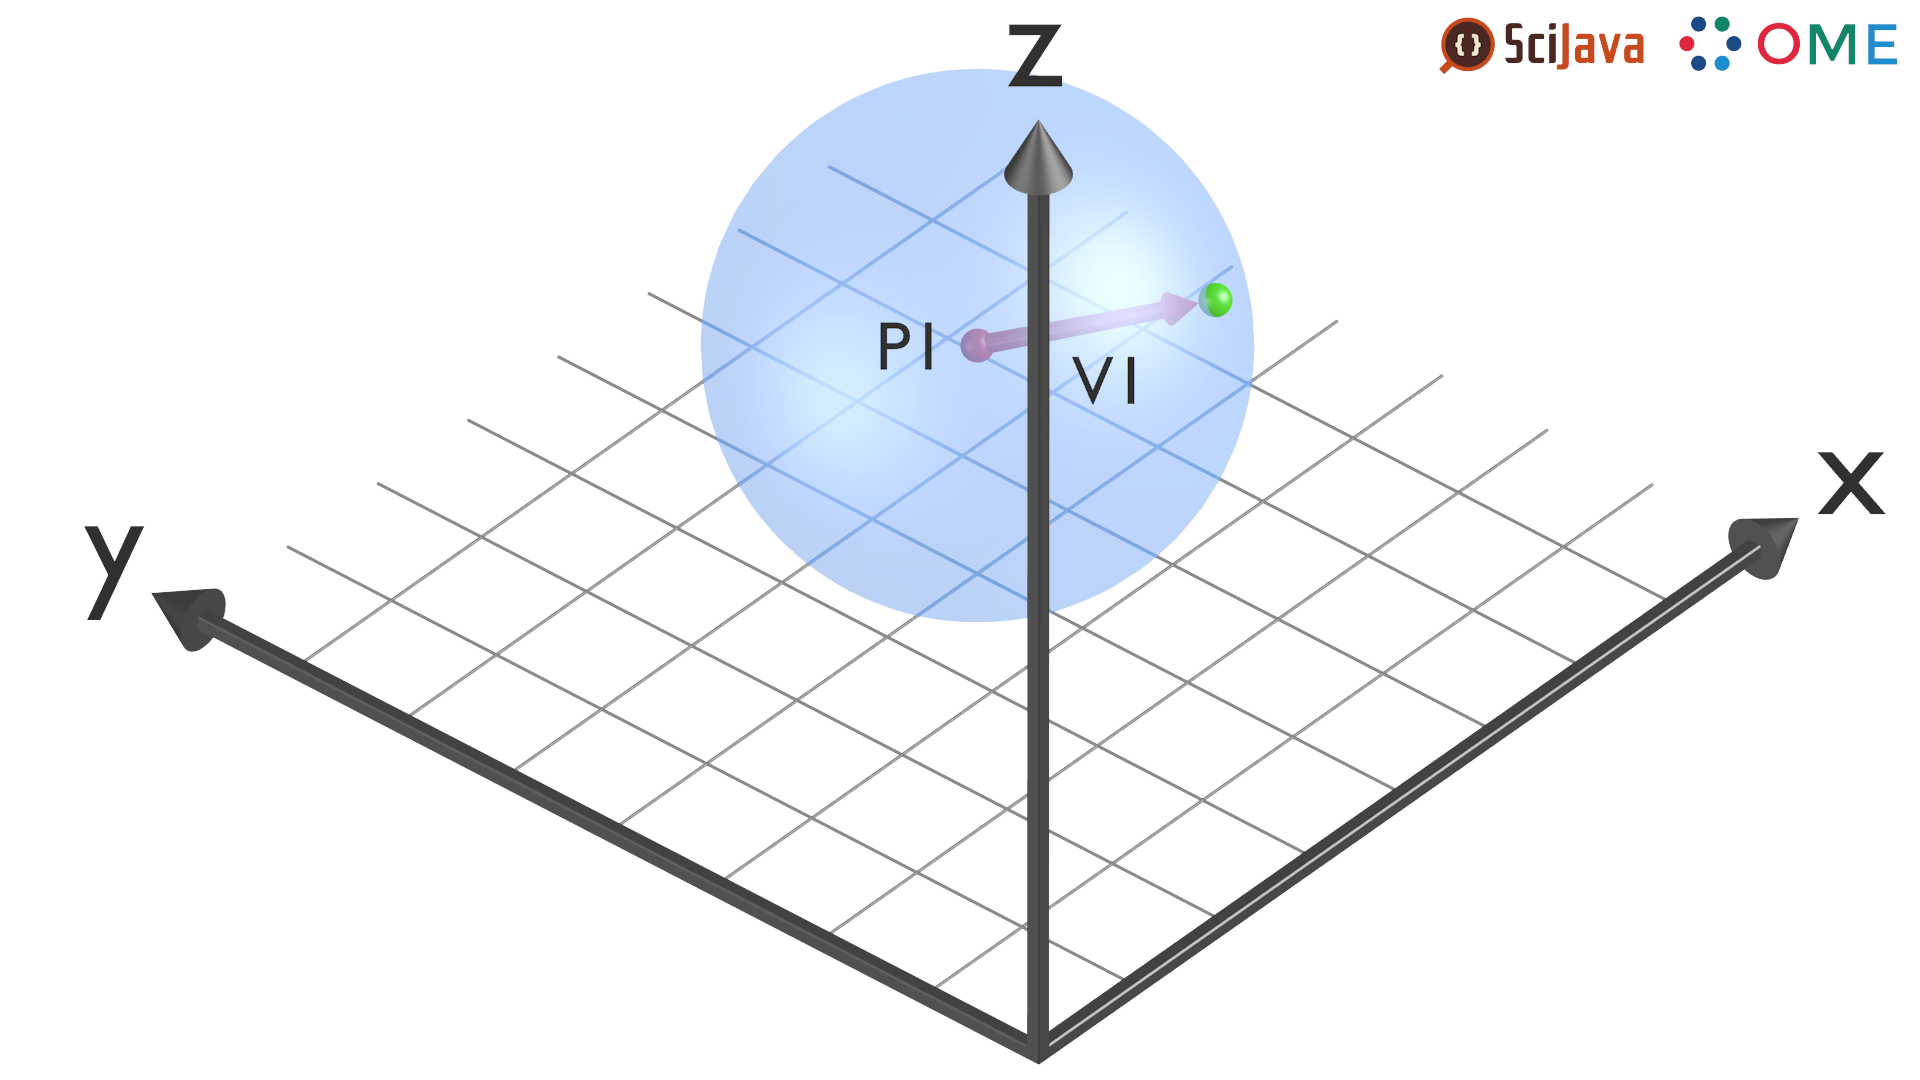
\includegraphics[width=\textwidth]{../images/3DspherePVR1.png}
\end{center}
}

\frame{
\frametitle{Shape serialisation example: sphere centre and radius}
\begin{center}
\begin{tabular}{lllS[table-format=2.5]l}
\textit{Name} & \textit{Type}    & \textit{Fundamental} & {\textit{Value}}  & \textit{Description} \\
\toprule
SID & ShapeID  & uint16      & 11       & Ellipsoid  \\
\cmidrule{3-5}
RID & RepID    & uint16      & 40       & RSphere3 \\
\cmidrule{3-5}
P1  & Vertex3D & double      & 16.0     & x \\
    &          & double      & 16.0     & y \\
    &          & double      &  8.0     & z \\
\cmidrule{3-5}
V1  & Vector3D & double      &  1.71653 & x \\
    &          & double      &  9.28585 & y \\
    &          & double      & 11.39716 & z
\end{tabular}
\\
\bigskip
Total size: 68 bytes.
\end{center}
}

\subsection{Shape relationships}

\frame{
  \frametitle{Shapes and canonical representations}
  \begin{center}
    \includegraphics[width=0.7\textwidth]{../gen/inherit-simple}
  \end{center}
}

{
  \setbeamertemplate{background}{
    \vbox to \paperheight{\vfil\hbox to \paperwidth{\hfil\includegraphics[width=0.98\paperwidth]{../gen/inherit}\hfil}\vfil}
  }
  \frame{
    \frametitle{Shapes and all representations}
  }
}

\subsection{Nested/stacked shapes and transformations}

\begin{frame}[fragile]
  \frametitle{Shapes and transformations can stack}
  \begin{center}
\begin{verbatim}
AffineTransform {
    Transform1
    Group {
        AffineTransform {
            Transform2   
            Set {
                Shape1,
                Shape2
                AffineTransform {
                    Transform3
                    Shape3
                }
            }
        }
    }
}
\end{verbatim}
  \end{center}
\end{frame}

\section{Masks}

\frame{
\begin{itemize}
  \item Conversion of shape to bitmasks and greymasks
\end{itemize}
  \frametitle{Bitmasks and greymasks}
  \centering
  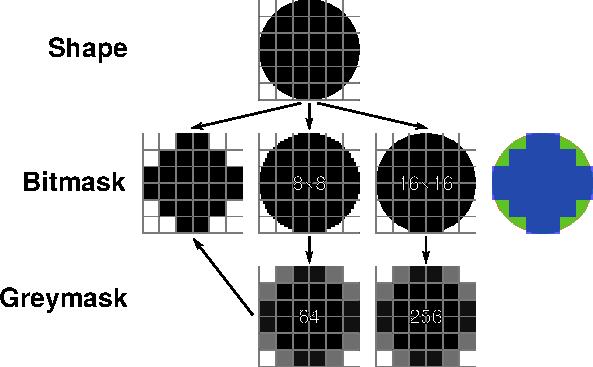
\includegraphics[width=0.8\textwidth]{../images/greymap}
\begin{itemize}
  \item Optimal storage for bitmasks?
  \item Alignment of masks with the image pixel grid?
\end{itemize}
}

\frame{
  \frametitle{Set operations on bitmasks}
  \centering
  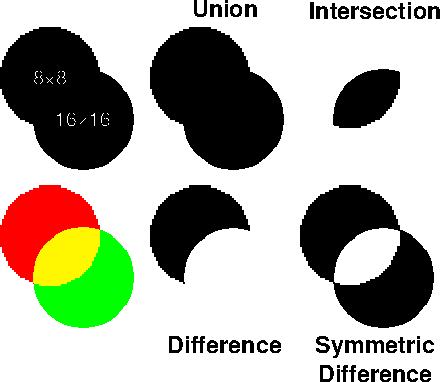
\includegraphics[width=0.75\textwidth]{../images/greymap2}
  \\
  \bigskip
  The resulting masks can be converted to a lower resolution greymask or
  bitmask.
}


\section{Drawing}

\frame{
  \frametitle{Drawing}
  \begin{itemize}
    \item Needs to be toolkit-independent
    \item All shapes draw using their canonical representation; one
      codepath for each shape type.
    \item Shapes reduce to:
      \begin{itemize}
        \item Bitmask
        \item Greymask
        \item Mesh
      \end{itemize}
    \item Viewers can all view masks or meshes in 2D or 3D
    \item OpenGL viewers can render meshes in 2D or 3D
    \item jHotDraw can render vectors where possible; unsupported
      complex types can be rendered in terms of simpler primitives
    \item There may be potentical loss of precision when converting;
      these forms are for visualisation only, not analysis.
  \end{itemize}
}

\section{Editing}

\frame{
  \frametitle{Editing}
  \begin{itemize}
    \item Edit in terms of the underlying shape representation
    \item Use the canonical representation where the original
      representation is not usable
    \item Edit in pixel, physical or other coordinate system
    \item Editing nodes and constraints specified by representation
    \item Possible to view the ROI as a treeview of nested shapes, and
      edit the properties of nodes in the view
  \end{itemize}
}

\section{Further discussion}

\frame{
  \frametitle{Outstanding questions}
  \begin{itemize}
    \item Grouping: what is a ``ROI'' cf. ``Shape'' or group/set of shapes?  What is the boundary between a shape and a ROI?
    \item Rounded rectangles.  Support as primitive or compound shape?
      \begin{itemize}
      \item Danger of infringing \emph{registered
        design No. 0000181607-0001}!
      \end{itemize}
    \item Efficient mask storage: labellings, etc.  Logic behind the
      different mechanisms?  Convenience?
    \item Shape properties: what is currently in the different models?
    \item State machine properties for evaluating ROIs
    \item Dimension conventions: are shapes present in all
      absent/unspecified dimensions?
  \end{itemize}
}

\frame{
  \frametitle{Needed work}
  \begin{itemize}
  \item Agree on list of shape primitives
  \item Agree on list of representation primitives
  \item Agree on most appropriate canonical shape representations
  \item For each shape type, specify:
    \begin{itemize}
    \item Mask conversion rules
    \item Measurements
    \item Editing rules
    \item Drawing behaviour (greymap, jHotDraw, OpenGL etc.)
    \end{itemize}
  \item Write code!
  \item Integrate and test code with programs using the ROI model
  \end{itemize}
}

\section*{Acknowledgements}

\frame{
  \frametitle{Acknowledgements}
  \parbox[t]{0.45\textwidth}{
    \begin{itemize}
    \item OME, Dundee
      \begin{itemize}
      \item Jason Swedlow
      \item Chris Allan
      \item Jean-Marie Burel
      \item Will Moore
      \item Andrew Patterson
      \end{itemize}
    \item OME, Edinburgh / Harvard Medical School
      \begin{itemize}
      \item Sébastien Besson
      \end{itemize}
    \end{itemize}
  }

  \begin{center}
    
      \parbox{0.25\textwidth}{
        
\includegraphics[width=0.2\textwidth]{../images/dundee}}\hfill
      \parbox{0.3\textwidth}{
      
\includegraphics[width=0.3\textwidth]{../images/wellcome}}\hfill
      \parbox{0.25\textwidth}{
        \hfill
\includegraphics[width=0.25\textwidth]{../images/scijava}\\
        \smallskip
        \hfill
\includegraphics[width=0.25\textwidth]{../images/ome}
      }
  \end{center}
}

\end{document}
